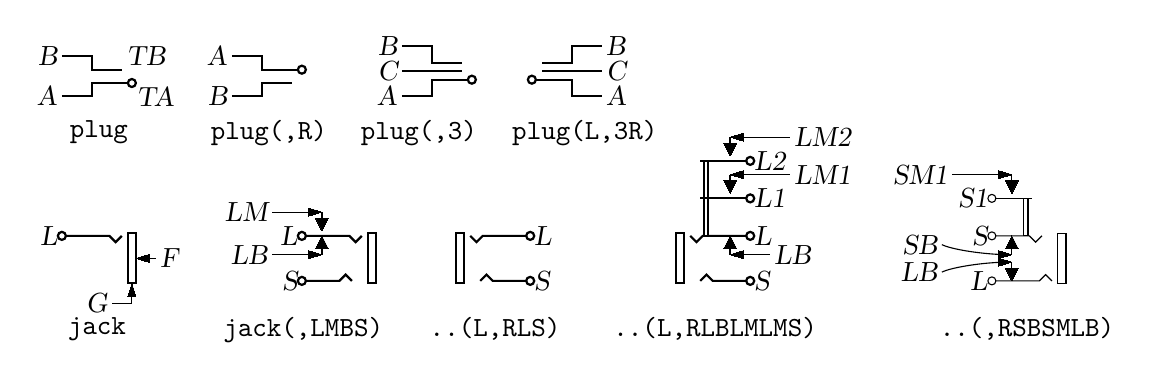
\begin{tikzpicture}[scale=2.54]
% dpic version 2020.03.01 option -g for TikZ and PGF 1.01
\ifx\dpiclw\undefined\newdimen\dpiclw\fi
\global\def\dpicdraw{\draw[line width=\dpiclw]}
\global\def\dpicstop{;}
\dpiclw=0.8bp
\dpiclw=0.8bp
\dpicdraw (0.127778,-0.061111)
 --(0.277778,-0.061111)
 --(0.277778,0.005556)
 --(0.477778,0.005556)\dpicstop
\dpicdraw[fill=white](0.477778,0.005556) circle (0.007874in)\dpicstop
\dpicdraw (0.127778,0.138889)
 --(0.277778,0.138889)
 --(0.277778,0.072222)
 --(0.427778,0.072222)\dpicstop
\draw (0.127778,-0.061111) node[left=-2bp]{\sl A};
\draw (0.127778,0.138889) node[left=-2bp]{\sl B};
\draw (0.427778,0.072222) node[above right=-2bp]{\sl TB};
\draw (0.477778,0.005556) node[below right=-2bp]{\sl TA};
\dpicdraw (0.977778,0.138889)
 --(1.127778,0.138889)
 --(1.127778,0.072222)
 --(1.327778,0.072222)\dpicstop
\dpicdraw[fill=white](1.327778,0.072222) circle (0.007874in)\dpicstop
\dpicdraw (0.977778,-0.061111)
 --(1.127778,-0.061111)
 --(1.127778,0.005556)
 --(1.277778,0.005556)\dpicstop
\draw (0.977778,0.138889) node[left=-2bp]{\sl A};
\draw (0.977778,-0.061111) node[left=-2bp]{\sl B};
\dpicdraw (1.827778,-0.061111)
 --(1.977778,-0.061111)
 --(1.977778,0.022222)
 --(2.177778,0.022222)\dpicstop
\dpicdraw[fill=white](2.177778,0.022222) circle (0.007874in)\dpicstop
\dpicdraw (1.827778,0.063889)
 --(2.127778,0.063889)\dpicstop
\dpicdraw (1.827778,0.188889)
 --(1.977778,0.188889)
 --(1.977778,0.105556)
 --(2.127778,0.105556)\dpicstop
\draw (1.827778,-0.061111) node[left=-2bp]{\sl A};
\draw (1.827778,0.188889) node[left=-2bp]{\sl B};
\draw (1.827778,0.063889) node[left=-2bp]{\sl C};
\dpicdraw (2.827778,-0.061111)
 --(2.677778,-0.061111)
 --(2.677778,0.022222)
 --(2.477778,0.022222)\dpicstop
\dpicdraw[fill=white](2.477778,0.022222) circle (0.007874in)\dpicstop
\dpicdraw (2.827778,0.063889)
 --(2.527778,0.063889)\dpicstop
\dpicdraw (2.827778,0.188889)
 --(2.677778,0.188889)
 --(2.677778,0.105556)
 --(2.527778,0.105556)\dpicstop
\draw (2.827778,-0.061111) node[right=-2bp]{\sl A};
\draw (2.827778,0.188889) node[right=-2bp]{\sl B};
\draw (2.827778,0.063889) node[right=-2bp]{\sl C};
\draw (0.312778,-0.161111) node[below=-2bp]{\tt plug};
\draw (1.162778,-0.161111) node[below=-2bp]{\tt plug(,R)};
\draw (1.912778,-0.161111) node[below=-2bp]{\tt plug(,3)};
\draw (2.742778,-0.161111) node[below=-2bp]{\tt plug(L,3R)};
\global\let\dpicshdraw=\dpicdraw\global\def\dpicdraw{}
\global\def\dpicstop{--}
\dpicshdraw[fill=white!100!black]
\dpicdraw (0.498611,-0.871242)
 --(0.498611,-0.746242)
 --(0.456944,-0.746242)
 --(0.456944,-0.996242)
 --(0.498611,-0.996242)
 --(0.498611,-0.871242)\dpicstop
cycle; \global\let\dpicdraw=\dpicshdraw\global\def\dpicstop{;}
\dpicdraw (0.427778,-0.758742)
 --(0.396528,-0.789992)
 --(0.365278,-0.758742)
 --(0.127778,-0.758742)\dpicstop
\dpicdraw[fill=white](0.127778,-0.758742) circle (0.007874in)\dpicstop
\dpiclw=0.4bp
\draw (0.127778,-0.758742) node[left=-2bp]{\sl L};
\filldraw[line width=0bp](0.565278,-0.851242)
 --(0.498611,-0.871242)
 --(0.565278,-0.891242) --cycle\dpicstop
\dpicdraw (0.517945,-0.871242)
 --(0.598611,-0.871242)\dpicstop
\draw (0.598611,-0.871242) node[right=-2bp]{\sl F};
\filldraw[line width=0bp](0.497778,-1.062909)
 --(0.477778,-0.996242)
 --(0.457778,-1.062909) --cycle\dpicstop
\dpicdraw (0.477778,-1.015576)
 --(0.477778,-1.096242)
 --(0.377778,-1.096242)\dpicstop
\draw (0.377778,-1.096242) node[left=-2bp]{\sl G};
\dpiclw=0.8bp
\global\let\dpicshdraw=\dpicdraw\global\def\dpicdraw{}
\global\def\dpicstop{--}
\dpicshdraw[fill=white!100!black]
\dpicdraw (1.698611,-0.871242)
 --(1.698611,-0.746242)
 --(1.656944,-0.746242)
 --(1.656944,-0.996242)
 --(1.698611,-0.996242)
 --(1.698611,-0.871242)\dpicstop
cycle; \global\let\dpicdraw=\dpicshdraw\global\def\dpicstop{;}
\dpicdraw (1.627778,-0.758742)
 --(1.596528,-0.789992)
 --(1.565278,-0.758742)
 --(1.327778,-0.758742)\dpicstop
\dpicdraw[fill=white](1.327778,-0.758742) circle (0.007874in)\dpicstop
\filldraw[line width=0bp](1.396528,-0.671242)
 --(1.427778,-0.733742)
 --(1.459028,-0.671242) --cycle\dpicstop
\dpicdraw (1.427778,-0.72132)
 --(1.427778,-0.639992)\dpicstop
\filldraw[line width=0bp](1.459028,-0.821242)
 --(1.427778,-0.758742)
 --(1.396528,-0.821242) --cycle\dpicstop
\dpicdraw (1.427778,-0.771165)
 --(1.427778,-0.852492)\dpicstop
\dpicdraw (1.577778,-0.983742)
 --(1.546528,-0.952492)
 --(1.515278,-0.983742)
 --(1.327778,-0.983742)\dpicstop
\dpicdraw[fill=white](1.327778,-0.983742) circle (0.007874in)\dpicstop
\dpiclw=0.4bp
\draw (1.327778,-0.758742) node[left=-2bp]{\sl L};
\filldraw[line width=0bp](1.361111,-0.659992)
 --(1.427778,-0.639992)
 --(1.361111,-0.619992) --cycle\dpicstop
\dpicdraw (1.408444,-0.639992)
 --(1.177778,-0.639992)\dpicstop
\draw (1.177778,-0.639992) node[left=-2bp]{\sl LM};
\filldraw[line width=0bp](1.361111,-0.872492)
 --(1.427778,-0.852492)
 --(1.361111,-0.832492) --cycle\dpicstop
\dpicdraw (1.408444,-0.852492)
 --(1.177778,-0.852492)\dpicstop
\draw (1.177778,-0.852492) node[left=-2bp]{\sl LB};
\draw (1.327778,-0.983742) node[left=-2bp]{\sl S};
\dpiclw=0.8bp
\global\let\dpicshdraw=\dpicdraw\global\def\dpicdraw{}
\global\def\dpicstop{--}
\dpicshdraw[fill=white!100!black]
\dpicdraw (2.098611,-0.871242)
 --(2.098611,-0.996242)
 --(2.140278,-0.996242)
 --(2.140278,-0.746242)
 --(2.098611,-0.746242)
 --(2.098611,-0.871242)\dpicstop
cycle; \global\let\dpicdraw=\dpicshdraw\global\def\dpicstop{;}
\dpicdraw (2.169444,-0.758742)
 --(2.200694,-0.789992)
 --(2.231944,-0.758742)
 --(2.469444,-0.758742)\dpicstop
\dpicdraw[fill=white](2.469444,-0.758742) circle (0.007874in)\dpicstop
\dpicdraw (2.219444,-0.983742)
 --(2.250694,-0.952492)
 --(2.281944,-0.983742)
 --(2.469444,-0.983742)\dpicstop
\dpicdraw[fill=white](2.469444,-0.983742) circle (0.007874in)\dpicstop
\dpiclw=0.4bp
\draw (2.469444,-0.758742) node[right=-2bp]{\sl L};
\draw (2.469444,-0.983742) node[right=-2bp]{\sl S};
\dpiclw=0.8bp
\global\let\dpicshdraw=\dpicdraw\global\def\dpicdraw{}
\global\def\dpicstop{--}
\dpicshdraw[fill=white!100!black]
\dpicdraw (3.198611,-0.871242)
 --(3.198611,-0.996242)
 --(3.240278,-0.996242)
 --(3.240278,-0.746242)
 --(3.198611,-0.746242)
 --(3.198611,-0.871242)\dpicstop
cycle; \global\let\dpicdraw=\dpicshdraw\global\def\dpicstop{;}
\dpicdraw (3.269444,-0.758742)
 --(3.300694,-0.789992)
 --(3.331944,-0.758742)
 --(3.569444,-0.758742)\dpicstop
\dpicdraw[fill=white](3.569444,-0.758742) circle (0.007874in)\dpicstop
\filldraw[line width=0bp](3.500694,-0.821242)
 --(3.469444,-0.758742)
 --(3.438194,-0.821242) --cycle\dpicstop
\dpicdraw (3.469444,-0.771165)
 --(3.469444,-0.852492)\dpicstop
\dpicdraw (3.319444,-0.571242)
 --(3.569444,-0.571242)\dpicstop
\dpicdraw[fill=white](3.569444,-0.571242) circle (0.007874in)\dpicstop
\global\let\dpicshdraw=\dpicdraw\global\def\dpicdraw{}
\global\def\dpicstop{--}
\dpicshdraw[fill=white!100!black]
\dpicdraw (3.339028,-0.664992)
 --(3.339028,-0.758742)
 --(3.359861,-0.758742)
 --(3.359861,-0.571242)
 --(3.339028,-0.571242)
 --(3.339028,-0.664992)\dpicstop
cycle; \global\let\dpicdraw=\dpicshdraw\global\def\dpicstop{;}
\filldraw[line width=0bp](3.438194,-0.483742)
 --(3.469444,-0.546242)
 --(3.500694,-0.483742) --cycle\dpicstop
\dpicdraw (3.469444,-0.53382)
 --(3.469444,-0.452492)\dpicstop
\dpicdraw (3.319444,-0.383742)
 --(3.569444,-0.383742)\dpicstop
\dpicdraw[fill=white](3.569444,-0.383742) circle (0.007874in)\dpicstop
\global\let\dpicshdraw=\dpicdraw\global\def\dpicdraw{}
\global\def\dpicstop{--}
\dpicshdraw[fill=white!100!black]
\dpicdraw (3.339028,-0.477492)
 --(3.339028,-0.571242)
 --(3.359861,-0.571242)
 --(3.359861,-0.383742)
 --(3.339028,-0.383742)
 --(3.339028,-0.477492)\dpicstop
cycle; \global\let\dpicdraw=\dpicshdraw\global\def\dpicstop{;}
\filldraw[line width=0bp](3.438194,-0.296242)
 --(3.469444,-0.358742)
 --(3.500694,-0.296242) --cycle\dpicstop
\dpicdraw (3.469444,-0.34632)
 --(3.469444,-0.264992)\dpicstop
\dpicdraw (3.319444,-0.983742)
 --(3.350694,-0.952492)
 --(3.381944,-0.983742)
 --(3.569444,-0.983742)\dpicstop
\dpicdraw[fill=white](3.569444,-0.983742) circle (0.007874in)\dpicstop
\dpiclw=0.4bp
\draw (3.569444,-0.571242) node[right=-2bp]{\sl L1};
\filldraw[line width=0bp](3.536111,-0.432492)
 --(3.469444,-0.452492)
 --(3.536111,-0.472492) --cycle\dpicstop
\dpicdraw (3.488778,-0.452492)
 --(3.769444,-0.452492)\dpicstop
\draw (3.769444,-0.452492) node[right=-2bp]{\sl LM1};
\draw (3.569444,-0.383742) node[right=-2bp]{\sl L2};
\filldraw[line width=0bp](3.536111,-0.244992)
 --(3.469444,-0.264992)
 --(3.536111,-0.284992) --cycle\dpicstop
\dpicdraw (3.488778,-0.264992)
 --(3.769444,-0.264992)\dpicstop
\draw (3.769444,-0.264992) node[right=-2bp]{\sl LM2};
\draw (3.569444,-0.983742) node[right=-2bp]{\sl S};
\draw (3.569444,-0.758742) node[right=-2bp]{\sl L};
\filldraw[line width=0bp](3.536111,-0.832492)
 --(3.469444,-0.852492)
 --(3.536111,-0.872492) --cycle\dpicstop
\dpicdraw (3.488778,-0.852492)
 --(3.669444,-0.852492)\dpicstop
\draw (3.669444,-0.852492) node[right=-2bp]{\sl LB};
\global\let\dpicshdraw=\dpicdraw\global\def\dpicdraw{}
\global\def\dpicstop{--}
\dpicshdraw[fill=white!100!black]
\dpicdraw (5.148611,-0.871242)
 --(5.148611,-0.746242)
 --(5.106944,-0.746242)
 --(5.106944,-0.996242)
 --(5.148611,-0.996242)
 --(5.148611,-0.871242)\dpicstop
cycle; \global\let\dpicdraw=\dpicshdraw\global\def\dpicstop{;}
\dpicdraw (5.077778,-0.983742)
 --(5.046528,-0.952492)
 --(5.015278,-0.983742)
 --(4.777778,-0.983742)\dpicstop
\dpicdraw[fill=white](4.777778,-0.983742) circle (0.007874in)\dpicstop
\filldraw[line width=0bp](4.846528,-0.921242)
 --(4.877778,-0.983742)
 --(4.909028,-0.921242) --cycle\dpicstop
\dpicdraw (4.877778,-0.97132)
 --(4.877778,-0.889992)\dpicstop
\dpicdraw (5.027778,-0.758742)
 --(4.996528,-0.789992)
 --(4.965278,-0.758742)
 --(4.777778,-0.758742)\dpicstop
\dpicdraw[fill=white](4.777778,-0.758742) circle (0.007874in)\dpicstop
\filldraw[line width=0bp](4.909028,-0.821242)
 --(4.877778,-0.758742)
 --(4.846528,-0.821242) --cycle\dpicstop
\dpicdraw (4.877778,-0.771165)
 --(4.877778,-0.852492)\dpicstop
\dpicdraw (4.977778,-0.571242)
 --(4.777778,-0.571242)\dpicstop
\dpicdraw[fill=white](4.777778,-0.571242) circle (0.007874in)\dpicstop
\global\let\dpicshdraw=\dpicdraw\global\def\dpicdraw{}
\global\def\dpicstop{--}
\dpicshdraw[fill=white!100!black]
\dpicdraw (4.958194,-0.664992)
 --(4.958194,-0.571242)
 --(4.937361,-0.571242)
 --(4.937361,-0.758742)
 --(4.958194,-0.758742)
 --(4.958194,-0.664992)\dpicstop
cycle; \global\let\dpicdraw=\dpicshdraw\global\def\dpicstop{;}
\filldraw[line width=0bp](4.846528,-0.483742)
 --(4.877778,-0.546242)
 --(4.909028,-0.483742) --cycle\dpicstop
\dpicdraw (4.877778,-0.53382)
 --(4.877778,-0.452492)\dpicstop
\draw (4.777778,-0.983742) node[left=-2bp]{\sl L};
\draw (4.777778,-0.758742) node[left=-2bp]{\sl S};
\draw (4.777778,-0.571242) node[left=-2bp]{\sl S1};
\filldraw[line width=0bp](4.811111,-0.472492)
 --(4.877778,-0.452492)
 --(4.811111,-0.432492) --cycle\dpicstop
\dpicdraw (4.858444,-0.452492)
 --(4.577778,-0.452492)\dpicstop
\draw (4.577778,-0.452492) node[left=-2bp]{\sl SM1};
\filldraw[line width=0bp](4.811111,-0.909992)
 --(4.877778,-0.889992)
 --(4.811111,-0.869992) --cycle\dpicstop
\dpicdraw (4.858444,-0.889992)
 ..controls (4.743111,-0.889992) and (4.577778,-0.914992)
 ..(4.527778,-0.939992)\dpicstop
\draw (4.527778,-0.939992) node[left=-2bp]{\sl LB};
\filldraw[line width=0bp](4.811111,-0.872492)
 --(4.877778,-0.852492)
 --(4.811111,-0.832492) --cycle\dpicstop
\dpicdraw (4.858444,-0.852492)
 ..controls (4.743111,-0.852492) and (4.577778,-0.827492)
 ..(4.527778,-0.802492)\dpicstop
\draw (4.527778,-0.802492) node[left=-2bp]{\sl SB};
\dpiclw=0.8bp
\draw (0.303194,-1.146242) node[below=-2bp]{\tt jack};
\draw (1.334306,-1.146242) node[below=-2bp]{\tt jack(,LMBS)};
\draw (2.294028,-1.146242) node[below=-2bp]{\tt ..(L,RLS)};
\draw (3.394028,-1.146242) node[below=-2bp]{\tt ..(L,RLBLMLMS)};
\draw (4.953194,-1.146242) node[below=-2bp]{\tt ..(,RSBSMLB)};
\end{tikzpicture}
\vspace*{-0.5\baselineskip}
